% <Diagram title> -- version <NN>.
%
% <One paragraph: what the diagram shows and where it came from (a
% whiteboard sketch, a module, a design discussion). If this is v02+, say
% what changed relative to the previous version.>
%
% Layout (top to bottom):
%   1. inputs band      -- <external inputs>
%   2. main pipeline    -- <A -> B -> C>
%   3. intermediate data -- <data products>; each enters from the stage that
%                          produces it and loops back up to the stage that
%                          consumes it
%   4. outputs band     -- <final outputs>
%
% Abbreviations:
%   <AB> = <meaning>
%
% Build: pdflatex <file>.tex
\documentclass[tikz,border=12pt]{standalone}
\usepackage{amsmath,amssymb}
\usetikzlibrary{arrows.meta,positioning,fit,backgrounds,calc}

% ---- Palette: one colour per node role, defined once --------------------
\definecolor{inputc}{RGB}{33,102,172}   % external inputs
\definecolor{procc}{RGB}{64,64,64}      % processing stages, arrows
\definecolor{llmc}{RGB}{118,42,131}     % a highlighted stage type (e.g. LLM)
\definecolor{datac}{RGB}{1,133,113}     % intermediate data
\definecolor{outc}{RGB}{178,24,43}      % final outputs, open-question marks

\tikzset{
  font=\sffamily\small,
  >={Stealth[length=2.4mm]},
  flow/.style={->, thick, draw=procc},
  box/.style={draw, thick, rounded corners=3pt, minimum height=9mm,
              minimum width=22mm, align=center},
  input/.style={box, draw=inputc, fill=inputc!8, minimum width=18mm,
                minimum height=12mm},
  process/.style={box, draw=procc, fill=procc!6},
  llm/.style={box, draw=llmc, fill=llmc!8},
  data/.style={box, draw=datac, fill=datac!8, rounded corners=9pt,
               minimum width=20mm},
  output/.style={box, draw=outc, fill=outc!8},
  band/.style={draw=#1!60, dashed, rounded corners=6pt, fill=#1!3,
               inner sep=10pt},
  bandlabel/.style={font=\sffamily\bfseries\footnotesize, text=#1,
                    anchor=south west},
  question/.style={font=\sffamily\bfseries\Large, text=outc},
}

% ---- Layout constants ----------------------------------------------------
% Horizontal offset of the entry/exit ports on a main-row node's bottom edge.
\newcommand{\port}{0.5}
% Vertical drop used when routing into and out of the data row.
\newcommand{\drop}{0.55}

\begin{document}
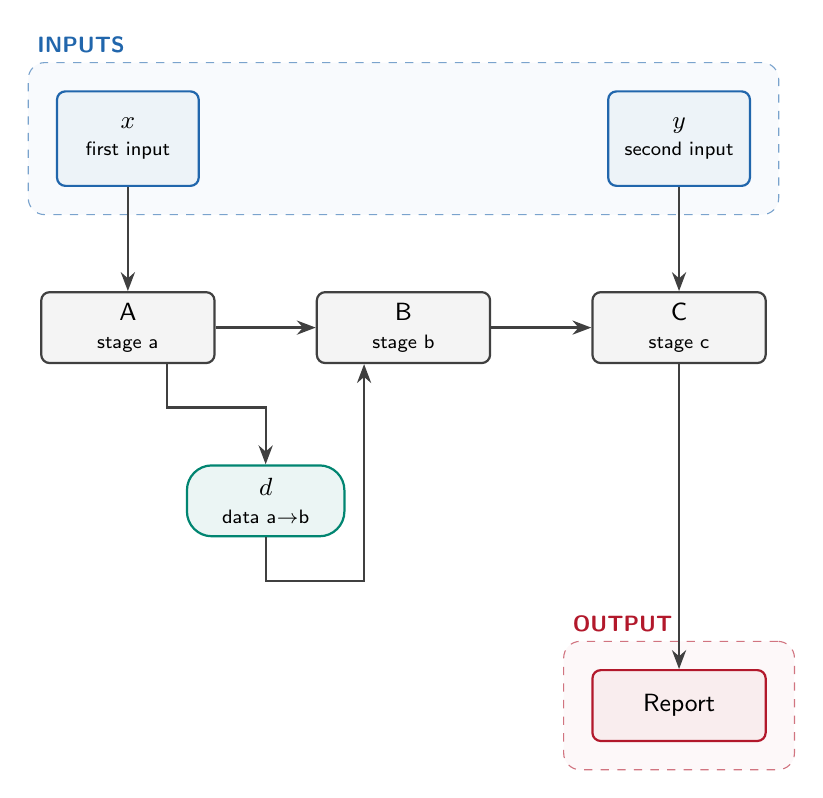
\begin{tikzpicture}

  % ---------------- Inputs (top) ----------------
  \node[input] (in1) at (0,0)   {$x$\\[-1pt]\scriptsize first input};
  \node[input] (in2) at (7.0,0) {$y$\\[-1pt]\scriptsize second input};

  % ---------------- Main row (3.5 units apart) ----------------
  \node[process] (a) at (0,-2.4)   {A\\[-1pt]\scriptsize stage a};
  \node[process] (b) at (3.5,-2.4) {B\\[-1pt]\scriptsize stage b};
  \node[process] (c) at (7.0,-2.4) {C\\[-1pt]\scriptsize stage c};

  % ---------------- Intermediate data row (midway between producer/consumer)
  \node[data] (d1) at (1.75,-4.6) {$d$\\[-1pt]\scriptsize data a$\to$b};

  % ---------------- Output (bottom) ----------------
  \node[output] (out) at (7.0,-7.2) {Report};

  % ---------------- Edges ----------------
  \draw[flow] (in1) -- (a);
  \draw[flow] (in2) -- (c);
  \draw[flow] (a) -- (b);
  \draw[flow] (b) -- (c);

  % Data row: enter from the top, exit from the bottom and loop up.
  % producer / data node / consumer
  \foreach \src/\dat/\dst in {a/d1/b} {
    \draw[flow] ($(\src.south)+(\port,0)$) -- ++(0,-\drop) -| (\dat.north);
    \draw[flow] (\dat.south) -- ++(0,-\drop) -| ($(\dst.south)+(-\port,0)$);
  }
  % A data node feeding a second consumer: branch off its exit line and
  % route one \drop lower so it passes under every other loop.
  % \coordinate (d1split) at ($(d1.south)+(0,-\drop)$);
  % \draw[flow] (d1split) -- ++(0,-\drop) -| (c.south);
  % \fill[procc] (d1split) circle (1.6pt);

  \draw[flow] (c) -- (out);

  % Open question on a stage:
  % \node[question, anchor=south] at ($(b.north)+(0,0.1)$) {?};

  % ---------------- Bands ----------------
  \begin{scope}[on background layer]
    \node[band=inputc, fit=(in1)(in2)] (inband) {};
    \node[band=outc,   fit=(out)] (outband) {};
  \end{scope}
  \node[bandlabel=inputc] at (inband.north west) {INPUTS};
  \node[bandlabel=outc]   at (outband.north west) {OUTPUT};

\end{tikzpicture}
\end{document}
